% FastLane final report -- ACL-style layout, single column, about 10-11 pages.
% The longer version with every fix and every intermediate run is fastlane_final_report_long.tex.
% Build: cd report/final && pdflatex fastlane_final_report && pdflatex fastlane_final_report
% Figures: .venv/bin/python results/final/final_tables.py && .venv/bin/python report/final/make_figures_final.py
\documentclass[11pt,a4paper]{article}

\usepackage[T1]{fontenc}
\usepackage[utf8]{inputenc}
\usepackage{times}
\renewcommand{\ttdefault}{lmtt}
\usepackage{microtype}
\usepackage[a4paper,top=2.2cm,bottom=2.2cm,left=2.3cm,right=2.3cm]{geometry}
\usepackage{graphicx}
\usepackage{booktabs}
\usepackage{tabularx}
\usepackage{array}
\usepackage{amsmath}
\usepackage{xcolor}
\usepackage{url}
\usepackage[small,labelfont=bf]{caption}
\usepackage{tikz}
\usetikzlibrary{positioning,arrows.meta,fit}
\PassOptionsToPackage{hyphens}{url}
\usepackage[hidelinks]{hyperref}
\newcommand{\hcell}[1]{\begin{tabular}[b]{@{}r@{}}#1\end{tabular}}  % right-aligned two-line table header

% ACL-like headings: section \large bold, subsection \normalsize bold, paragraph run-in bold.
\makeatletter
\renewcommand\section{\@startsection{section}{1}{\z@}{-2.0ex plus -0.5ex minus -0.2ex}{1.0ex plus 0.2ex}{\large\bfseries\raggedright}}
\renewcommand\subsection{\@startsection{subsection}{2}{\z@}{-1.6ex plus -0.5ex minus -0.2ex}{0.7ex plus 0.2ex}{\normalsize\bfseries\raggedright}}
\renewcommand\paragraph{\@startsection{paragraph}{4}{\z@}{1.0ex plus 0.5ex minus 0.2ex}{-1em}{\normalsize\bfseries}}
\makeatother
\setlength{\parindent}{1em}
\setlength{\emergencystretch}{2em}
\setlength{\parskip}{0pt}
\renewcommand{\topfraction}{0.85}\renewcommand{\bottomfraction}{0.6}\renewcommand{\textfraction}{0.1}
\renewcommand{\floatpagefraction}{0.75}\setcounter{topnumber}{3}\setcounter{bottomnumber}{2}\setcounter{totalnumber}{5}
\makeatletter\setlength{\@fptop}{0pt}\setlength{\@fpsep}{10pt plus 2pt}\makeatother
\setlength{\textfloatsep}{9pt plus 2pt minus 2pt}
\setlength{\floatsep}{7pt plus 2pt minus 2pt}
\setlength{\intextsep}{7pt plus 2pt minus 2pt}
\renewcommand{\arraystretch}{1.08}
\newcolumntype{L}{>{\raggedright\arraybackslash}X}
\newcommand{\cmd}[1]{{\small\ttfamily\def\_{\textunderscore\allowbreak}#1}}
\let\olditemize\itemize
\renewcommand{\itemize}{\olditemize\setlength{\itemsep}{1pt}\setlength{\parskip}{0pt}\setlength{\topsep}{2pt}}

\title{\Large\bfseries FastLane: A Voice Agent That Uses a Small Model for Easy Turns\\
and a Large Model Only for Hard Ones\\[4pt]
\normalsize\normalfont LMA Group Project 2026 --- Final Report (15 November 2026)}
\author{
  \textbf{Team: Chaturvedi and Sons}\\[4pt]
  \begin{tabular}{c@{\hspace{3em}}c@{\hspace{3em}}c}
  \textbf{Noel Alex Jacob} & \textbf{Aviral Tyagi} & \textbf{Sankalp Chaturvedi}\\
  2025201085 & 2025201086 & 2025201083\\[4pt]
  \multicolumn{3}{c}{\textbf{KSPSVLN Siddardha Kumar Kavuri}}\\
  \multicolumn{3}{c}{2025201061}
  \end{tabular}\\[6pt]
  {\small GitHub: \url{https://github.com/Sankalp0109/FastLane-Adaptive-Voice-Agent}}
}
\date{}

\begin{document}
\maketitle
\vspace{-1.5em}

\begin{abstract}
\noindent FastLane is a phone agent that books, changes and cancels movie tickets, bus tickets and restaurant tables for
Indian-English callers. A LoRA-tuned Qwen2.5-3B answers every turn first and passes only hard turns to a large API
model (gpt-oss-120b) or to staff; every action goes through a tool and policy gateway that enforces the booking rules
and a read-back confirmation in code. We built a deterministic practice booking system with 11 tools, a 360-call test
set with a simulated caller, a generator that produces training data by running an oracle agent through the real
orchestrator, and a local voice pipeline. Offline, fine-tuning lifts route accuracy from 89.1\% to 99.3\% and exact
tool arguments from 26.8\% to 99.0\%. In the final runs, FastLane succeeds in 108 of 120 calls (90.0\%) against 98
(81.7\%) for the large model alone (B1; $p=0.087$), with 78\% fewer large-model calls and no booking change the
caller did not confirm, while B1 makes such changes in 44 of 120 calls. FastLane is not faster (p95 6.8\,s vs.\
3.0\,s per turn), because one step of the local 3B model takes longer than a call to the hosted large model.
Ablations show that fine-tuning and rules in code matter most, and that a small model never trained on restaurants
does as well on them as the all-domains model (37 of 40 each).
\end{abstract}

% =====================================================================================================================
\section{Introduction}

A voice agent has about a second to reply before callers talk over it. Most agents send every turn to a large API
model, which adds latency and costs too much for a small cinema, bus operator or restaurant. Yet most turns in a
booking call are easy (a date, a seat count, a name, a ``yes'' to a read-back); only a few are hard (``next Friday'',
a sold-out show, a caller changing their mind, a request that breaks a rule). A wrong booking is worse than a slow
one, and recognisers often mishear Indian names, places and numbers. Our question is \emph{for each turn, which model
should reply}, judged on speed, correctness and safety together.

We study three research questions. \textbf{RQ1:} can a LoRA-tuned small model that both answers easy turns and
decides when to pass a turn on cut time per turn by $\geq$50\% without a real drop in booking success, compared with
a large-model-only agent? \textbf{RQ2:} does moving rules and routine work (dates, alternatives, policy checks) from
the prompt into code reduce large-model calls and unsafe bookings? \textbf{RQ3:} does a small model trained only on
movies and buses still work on restaurants? Seven hypotheses (H1--H7, Table~\ref{tab:hyp}) make these testable.

Our contributions are: (1) per-turn routing inside a tool-using dialogue in which the small model is its own router;
(2) a gateway that keeps booking rules, a read-back gate and grounding checks in code, outside both models;
(3) a training-data generator that runs an oracle agent through the real orchestrator, so training inputs match
inference byte for byte; (4) a 360-call evaluation of 12 systems (FastLane, 3 baselines, 8 ablations) that reports
success, latency and unconfirmed writes together, with every failed transcript read and labelled by cause. All code
(one Python package, about 10.6k lines, 218 tests), the training notebook, the result files of every run and a README
with the commands that reproduce every table are at \url{https://github.com/Sankalp0109/FastLane-Adaptive-Voice-Agent};
the trained adapters are at \url{https://huggingface.co/Sankalp0109/fastlane-adapters}.

% =====================================================================================================================
\section{Literature Review}\label{sec:lit}

\paragraph{Routing between models.} FrugalGPT~\cite{frugalgpt} queries a cascade of models of increasing cost and
stops when a scorer accepts the answer; Hybrid LLM~\cite{hybridllm} trains a router that predicts whether a small
model's answer is good enough; RouteLLM~\cite{routellm} learns such a router from preference data. All three choose
one model per \emph{question} on single-turn benchmarks with a separate router. FastLane routes \emph{per turn}
inside a long, tool-using dialogue, and the router is the small model itself (its route output and token
log-probabilities), so an easy turn pays for no routing call; baseline B3 tests a large model as the router.
Speculative decoding~\cite{specdec} is the other common way to make generation faster.

\paragraph{Task-oriented dialogue and tool use.} Earlier systems split belief tracking, policy and response
generation, trained on MultiWOZ~\cite{multiwoz}, Schema-Guided Dialogue~\cite{sgd} and Taskmaster-1~\cite{taskmaster};
SimpleTOD~\cite{simpletod} does all three as one sequence. Language models now act through tools: ReAct~\cite{react}
interleaves reasoning and actions, Toolformer~\cite{toolformer} learns when to call an API, and Gorilla~\cite{gorilla}
fine-tunes a model to write correct API calls. FastLane keeps the single-sequence style (route, slots, tool call and
reply in one JSON object) but trusts neither model with the rules: every change passes a gateway that checks them in
code. Policy answers follow retrieval-augmented generation~\cite{rag} with BM25~\cite{bm25}, and ablation A5 tests
step-by-step reasoning~\cite{cot} on hard turns.

\paragraph{Evaluating tool agents.} $\tau$-bench~\cite{taubench} scores tool agents against a gold final database
state with a language model as the simulated user; we adopt this protocol. $\tau$-bench does not measure latency, so
it rewards always using the largest model; we report speed, success and unsafe actions together, and count booking
changes the caller never confirmed separately, because a call can reach the gold state and still contain one.

\paragraph{Efficient fine-tuning and speech.} LoRA~\cite{lora} trains low-rank weight updates, and QLoRA~\cite{qlora}
does so on a 4-bit base, so a 3B model can be tuned on a free 16\,GB GPU. We tune Qwen2.5-3B-Instruct~\cite{qwen25},
serve it with MLX~\cite{mlx}, and use gpt-oss-120b~\cite{gptoss} as the large model. A voice agent is either a cascade
or a speech-to-speech model such as Moshi~\cite{moshi}; a cascade keeps tools and rules inspectable. Human turn gaps
are around 200\,ms~\cite{skantze}, so multi-second replies are noticed. Our cascade uses Silero VAD~\cite{silero},
Whisper~\cite{whisper} or Sarvam's Saarika~\cite{sarvam}, and Kokoro TTS~\cite{kokoro}; Svarah~\cite{svarah}, a
benchmark of English from speakers across India, is used to choose the recogniser.

% =====================================================================================================================
\section{Datasets Created and Used}\label{sec:data}

All dialogue data was created in a practice booking world (Section~\ref{sec:system}), so every call has an exact gold
outcome; the only public dataset used is Svarah. Table~\ref{tab:datasets} lists them.

\begin{table}[tbp]
\centering\small
\begin{tabularx}{\linewidth}{@{}>{\raggedright\arraybackslash}p{3.3cm}>{\raggedright\arraybackslash}p{3.9cm}L@{}}
\toprule
Dataset & Size & Use and source \\
\midrule
Practice booking world & 1,440 shows, 720 bus trips, 45 tables, 200 callers, 510 past bookings & SQLite, generated from a fixed seed; every call starts from the same snapshot \\
360-call test set & 120 per domain, 8 categories & scripted callers with gold final states and marked hard turns; never used for training \\
Training data (generated) & 645 calls; 3,153--3,722 train / 245--273 val steps per version & oracle agent run through the real orchestrator; five versions (Table~\ref{tab:data}); a movies+buses subset for A8 \\
Policy corpus + QA set & 25 documents ($\approx$21 pages); 67 questions & fares, refunds, FAQs, menus, festivals, old/new policy; retrieval evaluation \\
Svarah (AI4Bharat)~\cite{svarah} & 300 random test clips & real Indian-English speakers, 15+ first languages; recogniser comparison \\
TTS caller-line set & 142 clips & pilot caller lines spoken by 4 Kokoro voices; key-detail accuracy of recognisers \\
Round-trip noise set & 3,524 clips (1,762 lines $\times$ 2) & caller lines through TTS, a phone channel and Whisper; noise copies in data v5 \\
Routing-label sheet & 300 turns, 2 annotators & self / llm / staff labels to check the rule labels (Cohen's $\kappa$) \\
\bottomrule
\end{tabularx}
\caption{Datasets created and used. All except Svarah were created for this project. Converting Schema-Guided
Dialogue and Taskmaster-1, and recording the team's own voices, were planned but not done.}
\label{tab:datasets}
\end{table}

\paragraph{Test set.} 360 scripted calls, 120 per domain: simple book/change/cancel (120), relative dates and
festivals (45), sold out (45), policy questions (40), returning callers (40), change of mind (30), red flags and
out-of-scope requests (25), and rule-breaking requests such as waiving a deposit (15). Each script gives the persona,
goal, opening line, details revealed only when asked, marked hard turns and the gold final database state, which was
checked to be achievable. 10\% of calls get an injected tool failure. An LLM plays the caller in text.

\paragraph{Training-data generator.} Instead of an LLM teacher, both sides of each practice call are code: a
rule-based caller that follows a plan and an oracle agent that knows the ideal next step. The calls run through the
\emph{real} orchestrator and gateway, and every small-model call is stored as (exact input, ideal JSON output), so
training inputs match inference exactly and cost nothing to produce. Only calls that end in the planned final state
are kept (645 of 650). Routing targets follow the design: changed choices, ``my usual'' and refused details go to the
large model; red flags, deposit waivers and over-limit groups go to staff. Prompts are mixed across system variants
(FastLane 60\%, A2 15\%, A4 10\%, A6 5\%, A7 10\%) so one adapter serves all of them; escalation steps (about 5\%) are
repeated 3$\times$; data is split by call, 90/10. Table~\ref{tab:data} lists the five versions, each made to fix an
observed failure.

\begin{table}[tbp]
\centering\small
\begin{tabularx}{\linewidth}{@{}l r r L@{}}
\toprule
Data & Train & Val & What changed and why \\
\midrule
v1 & 3,722 & 273 & first version (3,095 self / 411 llm / 216 staff targets); rule-based speech-noise copies \\
v2 & 3,671 & 267 & spoken dates go in a slot and are resolved in code (all v1 errors were dates) \\
v3 & 3,671 & 267 & A2 only: the date the large model says back is stored as ISO (v2 labels were unlearnable) \\
v4 & 3,337 & 245 & callers give 0--5 details in any order, 35\% without the domain word (voice demo dropped details) \\
v5 & 3,153 & 245 & v4 calls; noise copies from a TTS$\rightarrow$phone$\rightarrow$STT round trip with a key-detail filter \\
\bottomrule
\end{tabularx}
\caption{Training data versions (all-domains set; steps).}
\label{tab:data}
\end{table}

\paragraph{Speech noise.} About 30\% of training steps get a copy with recogniser errors in the caller's lines. The
rule-based copies of v1--v4 (``four'' $\rightarrow$ ``for'') turned out to drop a key detail the target still
contained in 14.9\% of cases, which teaches the model to invent values. Data v5 instead speaks each caller line with a
Kokoro voice (half Hindi-accented), passes it through a phone channel (300--3400\,Hz, 12--30\,dB SNR) and transcribes
it with Whisper; a transcript is kept only if every key detail (places, films, dates, names, numbers, yes/no polarity)
survives. Of 3,524 clips (median WER 20\%), 55.7\% are usable.

\paragraph{Routing-label agreement.} Two team members labelled 300 practice turns as self / llm / staff without seeing
the rule label. They agree on 62\% (Cohen's $\kappa=0.17$~\cite{cohen}); against the rule labels $\kappa=0.65$ and
$0.42$. On plain bookings, dates and sold-out turns they agree on 127 of 128; the disagreement sits in design
decisions they were not given (``my usual'', changes of mind, deposit waivers, over-limit groups). The rule labels are
thus one consistent reading of the routing policy, and a written guideline would be needed for human agreement.

% =====================================================================================================================
\section{Methodology}\label{sec:method}

\subsection{System design}\label{sec:system}

\begin{figure}[tbp]
\centering
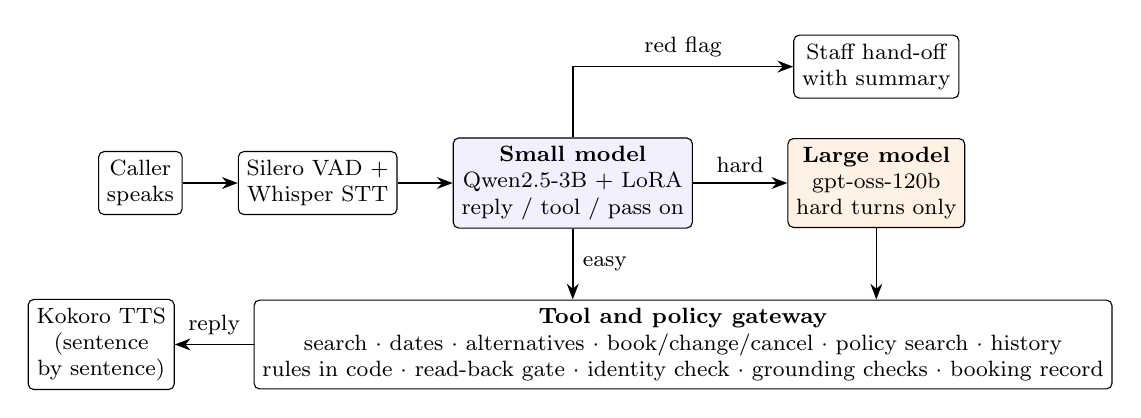
\begin{tikzpicture}[font=\footnotesize, node distance=6mm and 7mm,
  box/.style={draw, rounded corners=2pt, align=center, minimum height=8mm, inner sep=3pt, fill=white},
  arr/.style={-{Stealth[length=2mm]}, semithick}]
\node[box] (caller) {Caller\\speaks};
\node[box, right=of caller] (stt) {Silero VAD +\\Whisper STT};
\node[box, right=of stt, fill=blue!6] (small) {\textbf{Small model}\\Qwen2.5-3B + LoRA\\reply / tool / pass on};
\node[box, right=12mm of small, fill=orange!10] (large) {\textbf{Large model}\\gpt-oss-120b\\hard turns only};
\node[box, above=5mm of large] (staff) {Staff hand-off\\with summary};
\node[box, below=9mm of small, xshift=14mm] (gw) {\textbf{Tool and policy gateway}\\ search $\cdot$ dates $\cdot$ alternatives $\cdot$ book/change/cancel $\cdot$ policy search $\cdot$ history\\
rules in code $\cdot$ read-back gate $\cdot$ identity check $\cdot$ grounding checks $\cdot$ booking record};
\node[box, left=10mm of gw] (tts) {Kokoro TTS\\(sentence\\by sentence)};
\draw[arr] (caller) -- (stt);
\draw[arr] (stt) -- (small);
\draw[arr] (small) -- node[above]{hard} (large);
\draw[arr] (small.north) |- node[pos=0.75, above]{red flag} (staff.west);
\draw[arr] (small) -- node[right]{easy} (gw.north -| small);
\draw[arr] (large.south) -- (gw.north -| large);
\draw[arr] (gw) -- node[above]{reply} (tts);
\end{tikzpicture}
\caption{FastLane. Every caller turn goes to the tuned small model, which replies (optionally with a tool call),
passes the turn to the large model, or hands it to staff. Neither model writes to the booking system directly.}
\label{fig:arch}
\end{figure}

\paragraph{Practice world.} One SQLite database built from a fixed seed with a fixed ``now'' (Thursday 15 October
2026, so Dussehra and Diwali fall in the booking window): 4 cinemas, 9 films and 1,440 shows with seat maps; 6 bus
routes between Hyderabad and three cities with 720 trips; 3 restaurant branches with 45 tables; 200 callers with 510 past bookings. Some
shows, trips and slots are sold out on purpose. Each test call starts from the same snapshot.

\paragraph{Gateway and rules.} The gateway exposes 11 tools with validated arguments (search, date resolution,
alternatives, create/modify/cancel, lookup, caller history, policy search, SMS and hand-off). Rules are enforced in
code, not in the prompt: ticket and seat limits, change deadlines, bus passenger details, refund tiers, party limits
and deposits. A create, change or cancel first returns a read-back that must be spoken to the caller; the write
succeeds only after the caller confirms it in the next turn, and changes need the booking's phone number. Four rules
were added after observed failures: \emph{passenger source} (every bus passenger's name and age must have been said
by the caller or come from their history), \emph{grounding} (the booked venue and time must have been said by the
caller or offered by the agent), \emph{heard count} (a ticket count or party size must be a number the caller said)
and \emph{origin heard} (a bus search from a city other than Hyderabad needs the caller to have named it). There is
no payment tool.

\paragraph{Routing.} The small model outputs one JSON object: \cmd{route} (self / llm / staff), the slots heard this
turn, an optional tool call and the words to say. A turn goes to the large model when the small model routes it there
or its escalation score, $P(\text{llm})+P(\text{staff})$ at the route token, exceeds 0.5, and in code on a tool error,
no availability, a changed earlier choice, an unconfident policy match, a repeated tool call, a policy answer with
numbers or a ``no'' after a policy search, a refund figure given without a search, or a reply that claims a change the
gateway did not make. It goes to staff on the ``staff'' route or after two failed tool calls in a row. The large model
gets a typed booking record (shared by both models and the staff summary), the last turns and the same tools,
finishes the turn and returns control. Read-backs and goodbyes are templates that need no model call. Policy questions
use a BM25 index over 25 documents, with lookup started early on partial transcripts.

\paragraph{Models and serving.} Large model: \cmd{openai/gpt-oss-120b} on Groq (paid tier for the final runs, no
backup model, so every system sees the same large model); rate-limit waiting is logged separately and never counted
as model time. Simulated caller: Qwen2.5-7B, local. Small models, tuned and untuned, run as 4-bit MLX models (1.6\,GB)
on a 16\,GB Apple M4 behind an OpenAI-compatible server that returns log-probabilities.

\subsection{Fine-tuning}\label{sec:training}
QLoRA~\cite{qlora,lora} on one Kaggle T4: 4-bit NF4 base, rank 16, $\alpha=32$, dropout 0.05 on all seven projection
matrices, learning rate $2\cdot10^{-4}$ with cosine decay and 3\% warm-up, effective batch 16, 2 epochs, sequence
length 2,048, loss on the target JSON only. A run takes about 3.3\,h; validation loss flattens from about epoch 1.7
(v3: 0.0105, token accuracy 99.4\%). We trained all-domains adapters on data v1, v2, v3 and v5, and movies+buses
adapters on v2 and v5 for A8; the final runs use v3. Adapters are merged and converted to 4-bit MLX locally.
The tuned model gets a 643-token system prompt instead of 1,062, which shortens prefill.

\subsection{Failure-driven fixes}\label{sec:fixes}
Every change started from an observed failure (a crashed run, a failed test call, a voice-demo call or a wrong offline
step) and was written as a unit test where possible. After each new gateway rule, all 650 practice calls were
regenerated through the new code to confirm that the rule never blocks a correct booking (no training example
changed), so code fixes needed no retraining. Fixes were never applied in the middle of a comparison run; a fixed
system is reported as a separate run. We made 37 fixes in total; Table~\ref{tab:fixes} groups them by when they
were made.

\begin{table}[tbp]
\centering\small
\begin{tabularx}{\linewidth}{@{}>{\raggedright\arraybackslash}p{2.6cm}LL@{}}
\toprule
Where (fixes) & Typical failure & Fix \\
\midrule
Serving (10) & rate-limit waits counted as latency; training crash on bfloat16; a stale merged folder evaluated as ``v2'' & waits logged as \cmd{throttle\_ms}; float32 LoRA weights; merge from scratch with weight-hash check \\
Pilot v0 (7) & ``Friday 23rd'' booked on the 16th; ``10:00'' read as 10 PM; scorer missed correct answers & date and time parsing rules; Unicode normalisation in the scorer \\
Data (4) & all v1 errors were dates; rule noise contradicted targets & data v2--v5 (Table~\ref{tab:data}) \\
Pilot v3, voice (5) & invented passenger ``Caller (40)''; refund table misread; unrequested cinema & passenger-source and grounding rules; numeric policy answers to the large model \\
Before final (7) & misheard word booked as 4 tickets; baseline B1 booked twice; same search 4 times & heard-count rule; truthful tool descriptions without the gate; repeated call escalates \\
After final (4) & guessed bus origin; ``your booking was cancelled'' after a refused cancel; ``no parking'' against the text & origin-heard rule; completion-claim check; ``no'' policy answers escalate \\
\bottomrule
\end{tabularx}
\caption{The 37 fixes, grouped by when they were made.}
\label{tab:fixes}
\end{table}

% =====================================================================================================================
\section{Experiment Runs}\label{sec:eval}

\paragraph{Systems.} One configuration object defines all 12 systems (Table~\ref{tab:systems}). Baselines are other
ways to build the same agent; each ablation differs from FastLane in exactly one flag.

\begin{table}[tbp]
\centering\small
\begin{tabularx}{\linewidth}{@{}lL@{}}
\toprule
System & How it differs from FastLane \\
\midrule
FastLane & tuned small model on every turn; hard turns to the large model or staff; tools, gateway, record, early lookup, history \\
B1 & large model only, booking rules in the prompt (how most voice agents work) \\
B2 & untuned small model only; large model never used \\
B3 & the large model decides before every turn whether it is easy or hard \\
A1--A8 & no fine-tuning (A1); no date/alternative tools (A2); rules only in the prompt, no read-back (A3); no booking record (A4); no step-by-step reasoning for the large model (A5); no early lookup (A6); no caller history (A7); small model trained on movies+buses only, tested on restaurants (A8) \\
\bottomrule
\end{tabularx}
\caption{The 12 systems, all presets of one configuration.}
\label{tab:systems}
\end{table}

\paragraph{Runs.} Table~\ref{tab:allruns} lists the runs. The final runs (10 November) use adapter v3 and
gpt-oss-120b on Groq's paid tier for every system. FastLane and B1 run on a stratified sample of 120 test calls (40 per
domain, 15 per category); B2, B3 and A1--A7 run on a nested sample of 48. The samples contain the 24 calls used during
development, so 96 of the 120 calls were never seen before. A8 is a matched pair: all-domains and movies+buses
adapters, both on data v5, on the same 40 restaurant calls.

\begin{table}[tbp]
\centering\small
\begin{tabularx}{\linewidth}{@{}>{\raggedright\arraybackslash}p{3.1cm}L>{\raggedright\arraybackslash}p{4.2cm}@{}}
\toprule
Run & Systems and data & Purpose \\
\midrule
Retrieval & BM25 on 67 policy questions & choose retrieval thresholds \\
Recognisers & 3 recognisers ($\pm$ domain word list) on 300 Svarah clips and 142 booking lines & choose the recogniser \\
Offline step checks & untuned base and adapters v1--v5 on 245--267 held-out steps & model development; offline A1, A8 \\
Pilots (21--26 Oct) & FastLane, untuned vs.\ tuned small model, 24 calls & first end-to-end check \\
Development runs & all 12 systems on 24 calls; v3 vs.\ v5 & find failures and fix them \\
Final runs (10 Nov) & FastLane, B1 on 120; B2, B3, A1--A7 on 48; A8 pair on 40 & main comparison \\
After-fix run (10 Nov) & FastLane with four more fixes, same 120 calls & effect of fixes; run-to-run variation \\
\bottomrule
\end{tabularx}
\caption{Experiment runs. Final runs use one seed.}
\label{tab:allruns}
\end{table}

\paragraph{Metrics.} \emph{Success:} the bookings created or changed match one acceptable gold outcome exactly (plus
hand-off and policy-answer expectations), with Wilson 95\% intervals~\cite{wilson}. \emph{Speed:} model time per turn
(p50/p95), excluding rate-limit waiting. \emph{Cost:} share of turns and calls sent to the large model, tokens per
call. \emph{Safety:} calls with a booking change the caller never confirmed, rule-breaking writes, missed hand-offs.
Also router precision/recall on marked hard turns and invalid tool calls. Systems are compared on the same calls with
an exact McNemar test~\cite{mcnemar}. The \emph{offline step check} replays held-out training steps and compares the
output with the target JSON (valid JSON, route, escalation precision/recall, right tool, exact arguments); it needs no
large model or caller, so it is cheap and deterministic.

% =====================================================================================================================
\section{Ablations}\label{sec:ablations}

Each ablation is FastLane with one part removed, run on the same calls (Table~\ref{tab:ablations}).

\begin{table}[tbp]
\centering\small
\setlength{\tabcolsep}{4pt}
\begin{tabular}{@{}llllrrr@{}}
\toprule
System & Part removed or changed & Tests & Success & $p$ & \hcell{Large calls\\per call} & \hcell{Unconfirmed-\\change calls} \\
\midrule
FastLane & -- & -- & 46/48 & -- & 1.67 & 0 \\
A1 & fine-tuning of the small model & RQ1 & 21/48 & $<$0.001 & 1.88 & 0 \\
A2 & date and alternative tools & H4 & 41/48 & 0.13 & 3.35 & 0 \\
A3 & rules and read-back in code & H5 & 35/48 & 0.001 & 2.21 & 31 \\
A4 & booking record & RQ2 & 42/48 & 0.22 & 2.77 & 0 \\
A5 & reasoning on hard turns & -- & 44/48 & 0.63 & 1.71 & 0 \\
A6 & early lookup & H7 & 43/48 & 0.25 & 1.69 & 0 \\
A7 & caller history & -- & 45/48 & 1.00 & 2.33 & 0 \\
\midrule
FastLane (v5)$^\dagger$ & -- & -- & 37/40 & -- & 0.90 & 0 \\
A8$^\dagger$ & restaurants in the training data & H6, RQ3 & 37/40 & 1.00 & 1.82 & 0 \\
\bottomrule
\end{tabular}
\caption{Ablations in the final runs, each against FastLane on the same calls ($p$: exact McNemar test).
$^\dagger$Restaurant calls only, both adapters trained on data v5.}
\label{tab:ablations}
\end{table}

\paragraph{A1: no fine-tuning.} With the untuned Qwen2.5-3B, FastLane succeeds in only 21 of 48 calls: 17\% of its
tool calls are invalid, 18 calls reach the turn limit, and the model rarely passes a turn on (12.8\% of turns), so it
keeps turns it cannot do. Offline, fine-tuning lifts route accuracy from 89.1\% to 99.3\% and exact arguments from
26.8\% to 99.0\% (Table~\ref{tab:offline}). Fine-tuning is what makes the small model usable.

\paragraph{A2: no date and alternative tools.} The small model passes dates and sold-out shows on: the share of turns
sent to the large model doubles (21.0\% $\rightarrow$ 41.8\%), large-model calls per call double (1.67
$\rightarrow$ 3.35) and median model time per turn rises from 1.61 to 2.61\,s. Success falls to 41 of 48.

\paragraph{A3: rules only in the prompt.} With the same models but no gateway rules or read-back gate,
\textbf{31 of 48 calls (65\%) made a booking change the caller never confirmed}, and 9 writes broke a booking rule.
Success falls to 35 of 48, and 20 of the 35 successful calls contained an unconfirmed change, so success alone
understates the risk.

\paragraph{A4--A7.} None changes success significantly on 48 calls; the effect shows in large-model use. Without the
booking record (A4) the large model gets more turns (30.2\%; 2.77 calls per call). Without reasoning on hard turns
(A5) it writes less than half the output tokens with no measurable loss. Without caller history (A7) it is called
more often (2.33 per call). Early lookup (A6) saves under 10\,ms in total, since a BM25 search takes milliseconds.

\paragraph{A8: no restaurant training data.} Both adapters succeed in 37 of 40 restaurant calls (one call differs
each way); the movies+buses adapter makes twice the large-model calls (1.82 vs.\ 0.90). Offline, its routing transfers
(98.1\% route accuracy on restaurant steps) but argument filling does not (47.6\% exact): every error is the movie/bus
field \cmd{quantity} where restaurants need \cmd{party\_size}, which the gateway now accepts as an alias.

% =====================================================================================================================
\section{Evaluations}\label{sec:results}

\subsection{Offline step accuracy and retrieval}\label{sec:offline}
Table~\ref{tab:offline} compares the untuned base with the tuned versions on the same held-out steps and serving
stack. Every remaining v1 error involved a date, which led to data v2; v3 removed an unlearnable A2 label. The six
remaining v3 errors are minor (e.g.\ a change without a prior search). The BM25 retriever reaches Recall@3 0.967 and
top-1 0.817 on the 67 policy questions, and picks the current policy version over the old one every time; its
thresholds were tuned on the same set.

\begin{table}[tbp]
\centering\small
\begin{tabular}{@{}lrrrr@{\hspace{2em}}rr@{}}
\toprule
& \multicolumn{4}{c}{267 steps of data v2} & \multicolumn{2}{c}{267 steps of data v3} \\
\cmidrule(r{2em}){2-5}\cmidrule{6-7}
Metric & Untuned & v1 & v2 & & v2 & v3 \\
\midrule
Route accuracy & 89.1 & 96.6 & \textbf{98.9} & & 99.3 & 99.3 \\
Escalation precision & 46.2 & 100 & 96.0 & & 100 & 100 \\
Escalation recall & 23.1 & 65.4 & \textbf{92.3} & & 92.3 & 92.3 \\
Right tool & 49.8 & 96.7 & 96.7 & & 95.9 & \textbf{98.8} \\
Exact tool arguments & 26.8 & 90.5 & \textbf{92.5} & & 97.2 & \textbf{99.0} \\
p50 / p95 latency (s) & 2.20 / 7.55 & 2.22 / 4.83 & 2.22 / 4.51 & & 2.32 / 4.88 & 1.96 / 4.24 \\
\bottomrule
\end{tabular}
\caption{Offline step accuracy (\%) of the small model; same steps and serving stack within each block.}
\label{tab:offline}
\end{table}

\subsection{Final comparison}\label{sec:baselines}

\begin{table}[tbp]
\centering\footnotesize
\setlength{\tabcolsep}{3.2pt}
\resizebox{\linewidth}{!}{%
\begin{tabular}{@{}lrrrrrrrrr@{}}
\toprule
System & Calls & Success [95\% CI] & \hcell{FastLane,\\same calls} & \hcell{$p$\\(McNemar)} & \hcell{Large-model\\turns} & \hcell{Large calls\\per call} & \hcell{p50 / p95\\(s)} & \hcell{Invalid\\tool calls} & \hcell{Unconfirmed-\\change calls} \\
\midrule
\textbf{FastLane} & 120 & \textbf{90.0\%} [83--94] & -- & -- & 20.9\% & 1.76 & 1.67 / 6.81 & 1.2\% & \textbf{0} \\
B1 large only & 120 & 81.7\% [74--88] & 108 & 0.087 & 100\% & 8.02 & \textbf{1.04} / \textbf{3.01} & 0.6\% & 44 \\
\midrule
\textbf{FastLane} & 48 & \textbf{95.8\%} [86--99] & -- & -- & 21.0\% & 1.67 & 1.61 / 6.70 & 1.3\% & \textbf{0} \\
B1 large only & 48 & 81.2\% [68--90] & 46 & 0.065 & 100\% & 8.42 & \textbf{1.01} / \textbf{3.12} & 1.6\% & 19 \\
B2 untuned small & 48 & 29.2\% [18--43] & 46 & $<$0.001 & 0\% & 0 & 1.65 / 16.08 & 27.6\% & 0 \\
B3 large as router & 48 & 91.7\% [80--97] & 46 & 0.50 & 76.0\% & 6.94 & 1.66 / 7.66 & 0.8\% & 0 \\
A1 no fine-tuning & 48 & 43.8\% [31--58] & 46 & $<$0.001 & 12.8\% & 1.88 & 1.53 / 5.52 & 17.0\% & 0 \\
A2 no date tools & 48 & 85.4\% [73--93] & 46 & 0.13 & 41.8\% & 3.35 & 2.61 / 8.65 & 3.1\% & 0 \\
A3 rules in prompt & 48 & 72.9\% [59--83] & 46 & 0.001 & 27.8\% & 2.21 & 2.28 / 7.50 & 6.4\% & 31 \\
A4 no booking record & 48 & 87.5\% [75--94] & 46 & 0.22 & 30.2\% & 2.77 & 1.76 / 6.55 & 1.8\% & 0 \\
A5 no reasoning & 48 & 91.7\% [80--97] & 46 & 0.63 & 21.1\% & 1.71 & 1.70 / 7.18 & 1.3\% & 0 \\
A6 no early lookup & 48 & 89.6\% [78--96] & 46 & 0.25 & 19.7\% & 1.69 & 1.68 / 7.11 & 1.2\% & 0 \\
A7 no caller history & 48 & 93.8\% [83--98] & 46 & 1.00 & 24.7\% & 2.33 & 1.81 / 7.03 & 3.3\% & 0 \\
\midrule
FastLane, adapter v5 & 40$^\dagger$ & 92.5\% [80--97] & -- & -- & 15.1\% & 0.90 & 1.60 / 7.39 & 1.7\% & 0 \\
A8 movies+buses v5 & 40$^\dagger$ & 92.5\% [80--97] & 37 & 1.00 & 24.2\% & 1.82 & 1.76 / 7.54 & 2.6\% & 0 \\
\bottomrule
\end{tabular}}
\caption{Final runs (one seed; gpt-oss-120b on Groq for every system). ``FastLane, same calls'': FastLane's successes
on the system's calls; $p$: exact McNemar test. Unconfirmed-change calls: calls with a booking change the caller
never confirmed. $^\dagger$Restaurant calls only (matched pair for A8).}
\label{tab:baselines}
\end{table}

\begin{figure}[tbp]
\centering
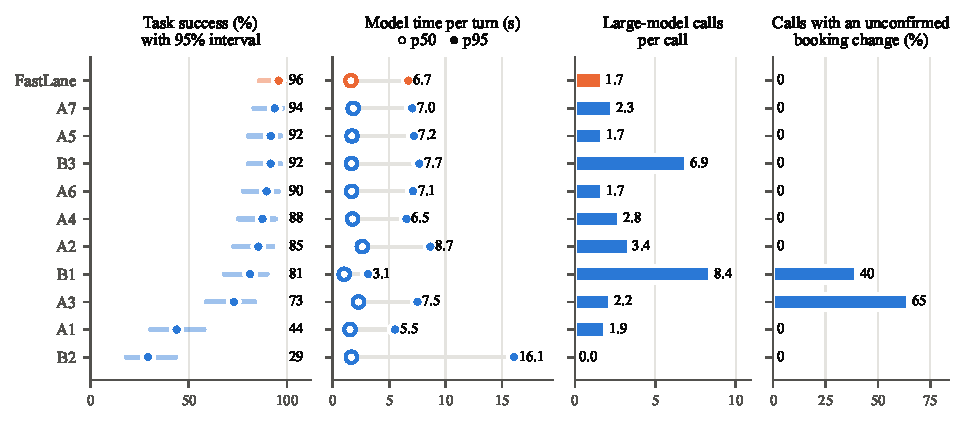
\includegraphics[width=0.92\linewidth]{figures/systems_final.pdf}
\caption{All systems on the same 48 calls, sorted by success: success with 95\% interval, model time per turn (p50
hollow, p95 filled), large-model calls per call, and share of calls with an unconfirmed change. FastLane in orange.}
\label{fig:systems}
\end{figure}

\paragraph{FastLane vs.\ the large model alone (B1).} On 120 calls FastLane succeeds in 108 (90.0\%) and B1 in 98
(81.7\%; Table~\ref{tab:baselines}). Paired, 19 calls succeed only with FastLane and 9 only with B1 ($p=0.087$): the
gap points one way but is not significant; on the 96 unseen calls it is 85 vs.\ 79. B1 loses most on sold-out calls
(8/15 vs.\ 14/15) and changes of mind. The clear difference is safety: B1 made 53 booking changes the caller never
confirmed, in 44 of 120 calls (37\%), 33 of which were still scored successful; 7 calls booked the same thing twice.
FastLane made none ($p=1.1\cdot10^{-13}$). FastLane also uses 78\% fewer large-model calls and 79\% fewer tokens
(4.2k vs.\ 19.5k per call).

\paragraph{Speed.} B1 is faster: p50 1.04\,s and p95 3.01\,s per turn against 1.67\,s and 6.81\,s. One gpt-oss-120b
call on Groq takes about a second, while one step of the 3B model on the laptop has a median of about 1.5\,s; booking
turns need two small-model steps (search, then read-back), and passed-on turns pay for both models. The proposal
assumed that a large API model adds 1--3\,s per turn; on Groq it adds about 1\,s, so on this setup routing to a local
model saves cost, quota and unsafe writes, not time.

\paragraph{Other baselines.} B3 (the large model as router) succeeds in 44 of 48 (FastLane 46; $p=0.5$) and, behind
the same gateway, makes no unsafe writes, but it sends 76\% of turns to the large model (4.2$\times$ FastLane's calls)
and catches hard turns no better (88.6\% each) at lower precision (42\% vs.\ 59\%). B2 (the untuned small model
alone) succeeds in 14 of 48, mostly where the right outcome is a refusal or hand-off; half its calls hit the turn
limit.

\subsection{Failure analysis and after-fix run}\label{sec:failures}
We read every failed transcript of FastLane (12) and B1 (22) and labelled the cause (Table~\ref{tab:flfail}). Half
of FastLane's failures come from the simulated caller, mostly by not changing its mind when the script says so; on
its own errors FastLane fails 5 of 120 calls, none with an unconfirmed change. Of B1's 22 failures, 17 end in wrong
bookings and 7 are duplicate bookings.

\begin{table}[tbp]
\centering\small
\begin{tabularx}{\linewidth}{@{}l>{\raggedright\arraybackslash}p{1.0cm}L@{}}
\toprule
Cause & Calls & What happened \\
\midrule
Simulated caller & 6 & the script says the caller changes the time and it never did (4); asked for an unplanned cancellation; kept asking for a bus type that does not exist \\
Scorer & 1 & ``a two-year-old does not need a ticket'' is correct, but the gold answer wants the age limit stated \\
Agent & 5 & searched from a bus origin the caller never said (2, a pattern in 4 training calls); said ``your booking was cancelled'' after the gateway refused; answered ``no parking'' against the retrieved text; a retrieval miss handed to staff \\
\bottomrule
\end{tabularx}
\caption{Causes of FastLane's 12 failures in the final run, from reading every transcript.}
\label{tab:flfail}
\end{table}

The first three agent error types led to four more fixes (origin-heard rule, completion-claim check, ``no'' policy
answers escalate, and a question containing ``confirm'' is no longer read as a yes). We reran FastLane with them on
the same 120 calls as a separate run. All four targeted calls now succeed and none of these error types recurs (the
origin rule refused 9 searches, each where the caller had not named the origin). Overall success was 105/120 (87.5\%),
not higher: 13 calls changed outcome, 8 of them with no fix involved, so run-to-run variation (Groq and the simulated
caller are not deterministic) is about $\pm$7\% of calls ($p=0.58$). Single-run differences of a few calls cannot show
the effect of a fix; the transcripts can.

\subsection{Speech}\label{sec:asr}
Table~\ref{tab:stt} compares recognisers. Sarvam is best on real Indian speech by a wide margin and 3$\times$ faster.
A domain word list lifts places on booking lines from 48\% to 97\% but raises WER on Svarah's general speech. Person
names are the weak spot for every recogniser (26--37\%). Measured on 245 validation steps, recogniser noise leaves
routing unchanged (98.8\%) but drops exact arguments of adapter v3 from 98.1\% to 94.3\%; adapter v5, trained on
round-trip noise, drops only from 95.9\% to 94.8\% and asks instead of inventing a time, but is slightly worse on
clean text, so the text-only final runs keep v3. In the browser voice demo (Silero VAD, Whisper large-v3-turbo on MLX,
the unchanged agent, Kokoro TTS sentence by sentence), the median time from the end of speech to the first reply
audio was 3.2\,s over an 8-turn booking.

\begin{table}[tbp]
\centering\small
\begin{tabular}{@{}lrr@{\hspace{2em}}rrrr@{}}
\toprule
& \multicolumn{2}{c}{Svarah (300 clips)} & \multicolumn{4}{c}{Booking lines, TTS (142 clips)} \\
\cmidrule(r{2em}){2-3}\cmidrule{4-7}
Recogniser & WER & s / clip & WER & Places & Names & Numbers \\
\midrule
Sarvam saarika:v2.5 (cloud) & \textbf{5.8} & \textbf{0.46} & 8.1 & 80.6 & \textbf{36.8} & 96.7 \\
Whisper large-v3-turbo (MLX) & 10.5 & 1.42 & 9.4 & 48.4 & 26.3 & 95.8 \\
\quad + domain word list & 14.9 & 1.40 & 8.0 & \textbf{96.8} & 26.3 & 94.2 \\
faster-whisper small.en (CPU) & 9.5 & 1.34 & 10.8 & 48.4 & 26.3 & \textbf{97.5} \\
\quad + domain word list & 12.3 & 1.50 & \textbf{7.8} & \textbf{96.8} & 26.3 & \textbf{97.5} \\
\bottomrule
\end{tabular}
\caption{Speech recognition: WER (\%), median time per clip, and key-detail accuracy (\%) on booking lines.}
\label{tab:stt}
\end{table}

\subsection{Hypotheses}\label{sec:status}
Table~\ref{tab:hyp} summarises the evidence. \emph{RQ1:} the tuned small model keeps quality and cuts large-model
calls by 78\%, but does not cut time per turn on our hardware. \emph{RQ2:} moving rules and routine work into code
halves large-model use (A2) and removes unconfirmed writes (A3, B1); this is the strongest result. \emph{RQ3:} a small
model never trained on restaurants does as well on them, at twice the large-model calls.

\begin{table}[tbp]
\centering\small
\begin{tabularx}{\linewidth}{@{}>{\raggedright\arraybackslash}p{3.6cm}>{\raggedright\arraybackslash}p{3.0cm}L@{}}
\toprule
Hypothesis & Expected & Evidence (final runs) \\
\midrule
H1 Routing is faster & p95 $\geq$50\% lower than B1 & \textbf{not supported}: p95 6.81\,s vs.\ 3.01\,s for B1 \\
H2 Quality holds & within 3 points of B1 & \textbf{supported}: 90.0\% vs.\ 81.7\% on 120 calls ($p=0.087$) \\
H3 Router catches hard turns & $\geq$90\% passed on & \textbf{partly}: 83.2\% on 120 calls (dates in code); 88.6\% on 48, same as B3; offline 92.3\% \\
H4 Tools cut large-model use & clearly lower & \textbf{supported}: without them (A2) calls per call 1.67 $\rightarrow$ 3.35 \\
H5 Rules in code are safer & fewer unsafe writes & \textbf{supported}: unconfirmed-change calls 0 vs.\ 31/48 (A3) and 44/120 (B1) \\
H6 Routing transfers & within 5 points & \textbf{supported}: 37/40 for both adapters on restaurants \\
H7 Early lookup hides delay & lower p95 on lookups & \textbf{not supported}: under 10\,ms saved in total \\
\bottomrule
\end{tabularx}
\caption{Hypotheses of the proposal and the evidence.}
\label{tab:hyp}
\end{table}

% =====================================================================================================================
\section{Limitations}
All results come from simulated callers and a practice booking system, with one seed: FastLane and B1 on 120 calls,
the other systems on 48 and A8 on 40. A rerun changed the outcome of 13 of 120 calls, so only the large gaps (A1, A3,
B2 and the unconfirmed changes) are reliable. Half of FastLane's failures come from the simulated caller not
following its script, so success rates are lower bounds, and none has been checked with real callers. The latency
comparison depends on hardware: the small model runs on a laptop, the large model on Groq's inference hardware. The
policy corpus has about 21 pages (60 were planned), and the retrieval thresholds were tuned on the questions used to
evaluate them. The round-trip noise uses synthetic voices. The routing labels are one design's policy that two
annotators without a guideline did not agree on ($\kappa=0.17$). Four training calls teach a guessed bus origin; the
gateway now blocks it, but the adapters were not retrained. Public dialogue corpora and real recordings were planned
but not used. \emph{Safety:} the system is a mock with no payment tool; every change needs a spoken read-back and the
booking's phone number; complaints and out-of-scope requests are handed to staff with a summary; the agent states that
it is automated; API keys stay in a local environment file.

\section{Conclusions}
A 3B model, fine-tuned on practice calls generated through the real agent, can answer most turns of a booking call
and pass the rest on: with the large model on about one turn in five, FastLane succeeds in 90\% of 120 simulated
calls, at least as often as the large model alone, with 78\% fewer large-model calls. The safety result is the
clearest: rules and read-back in code gave no booking change the caller had not confirmed, while the same rules in the
prompt left such changes in 37\% (B1) and 65\% (A3) of calls. The speed result is negative on our setup: a hosted
120B model on Groq answers faster than a 3B model on a laptop, so routing pays off in cost, quota and safety rather
than time. Most model errors came from the data, and reading every failed transcript told us more than the success
rate. Next steps are a faster small-model path (one step for search and read-back, speculative decoding), retraining
on regenerated data, a written routing guideline, and tests with real callers.

\paragraph{Code and reproducibility.} Code, the Kaggle training notebook, the result files of every run and a README
with the commands that reproduce every table and figure:
\url{https://github.com/Sankalp0109/FastLane-Adaptive-Voice-Agent}. Trained adapters:
\url{https://huggingface.co/Sankalp0109/fastlane-adapters}.

% =====================================================================================================================
\begin{thebibliography}{99}
\small
\setlength{\itemsep}{0pt}

\bibitem{frugalgpt} Lingjiao Chen, Matei Zaharia, and James Zou. 2024. FrugalGPT: How to use large language models
while reducing cost and improving performance. \emph{Transactions on Machine Learning Research}. arXiv:2305.05176.

\bibitem{hybridllm} Dujian Ding et al. 2024. Hybrid LLM: Cost-efficient and quality-aware query routing. In
\emph{Proceedings of ICLR}.

\bibitem{routellm} Isaac Ong et al. 2025. RouteLLM: Learning to route LLMs from preference data. In \emph{Proceedings
of ICLR}. arXiv:2406.18665.

\bibitem{specdec} Yaniv Leviathan, Matan Kalman, and Yossi Matias. 2023. Fast inference from transformers via
speculative decoding. In \emph{Proceedings of ICML}.

\bibitem{multiwoz} Pawe{\l} Budzianowski et al. 2018. MultiWOZ -- a large-scale multi-domain Wizard-of-Oz dataset for
task-oriented dialogue modelling. In \emph{Proceedings of EMNLP}.

\bibitem{sgd} Abhinav Rastogi, Xiaoxue Zang, Srinivas Sunkara, Raghav Gupta, and Pranav Khaitan. 2020. Towards
scalable multi-domain conversational agents: The schema-guided dialogue dataset. In \emph{Proceedings of AAAI}.

\bibitem{taskmaster} Bill Byrne et al. 2019. Taskmaster-1: Toward a realistic and diverse dialog dataset. In
\emph{Proceedings of EMNLP-IJCNLP}.

\bibitem{simpletod} Ehsan Hosseini-Asl, Bryan McCann, Chien-Sheng Wu, Semih Yavuz, and Richard Socher. 2020. A simple
language model for task-oriented dialogue. In \emph{Advances in NeurIPS}.

\bibitem{react} Shunyu Yao, Jeffrey Zhao, Dian Yu, Nan Du, Izhak Shafran, Karthik Narasimhan, and Yuan Cao. 2023.
ReAct: Synergizing reasoning and acting in language models. In \emph{Proceedings of ICLR}.

\bibitem{toolformer} Timo Schick et al. 2023. Toolformer: Language models can teach themselves to use tools. In
\emph{Advances in NeurIPS}.

\bibitem{gorilla} Shishir G. Patil, Tianjun Zhang, Xin Wang, and Joseph E. Gonzalez. 2024. Gorilla: Large language
model connected with massive APIs. In \emph{Advances in NeurIPS}.

\bibitem{rag} Patrick Lewis et al. 2020. Retrieval-augmented generation for knowledge-intensive NLP tasks. In
\emph{Advances in NeurIPS}.

\bibitem{bm25} Stephen Robertson and Hugo Zaragoza. 2009. The probabilistic relevance framework: BM25 and beyond.
\emph{Foundations and Trends in Information Retrieval}, 3(4):333--389.

\bibitem{cot} Jason Wei et al. 2022. Chain-of-thought prompting elicits reasoning in large language models. In
\emph{Advances in NeurIPS}.

\bibitem{taubench} Shunyu Yao, Noah Shinn, Pedram Razavi, and Karthik Narasimhan. 2025. $\tau$-bench: A benchmark for
tool-agent-user interaction in real-world domains. In \emph{Proceedings of ICLR}. arXiv:2406.12045.

\bibitem{lora} Edward J. Hu, Yelong Shen, Phillip Wallis, Zeyuan Allen-Zhu, Yuanzhi Li, Shean Wang, Lu Wang, and
Weizhu Chen. 2022. LoRA: Low-rank adaptation of large language models. In \emph{Proceedings of ICLR}.

\bibitem{qlora} Tim Dettmers, Artidoro Pagnoni, Ari Holtzman, and Luke Zettlemoyer. 2023. QLoRA: Efficient
finetuning of quantized LLMs. In \emph{Advances in NeurIPS}.

\bibitem{qwen25} Qwen Team. 2024. Qwen2.5 technical report. arXiv:2412.15115.

\bibitem{mlx} Awni Hannun, Jagrit Digani, Angelos Katharopoulos, and Ronan Collobert. 2023. MLX: Efficient and
flexible machine learning on Apple silicon. \url{https://github.com/ml-explore/mlx}.

\bibitem{gptoss} OpenAI. 2025. gpt-oss-120b \& gpt-oss-20b model card. arXiv:2508.10925.

\bibitem{moshi} Alexandre D{\'e}fossez et al. 2024. Moshi: A speech-text foundation model for real-time dialogue.
arXiv:2410.00037.

\bibitem{skantze} Gabriel Skantze. 2021. Turn-taking in conversational systems and human-robot interaction: A review.
\emph{Computer Speech \& Language}, 67:101178.

\bibitem{silero} Silero Team. 2024. Silero VAD: pre-trained voice activity detector.
\url{https://github.com/snakers4/silero-vad}.

\bibitem{whisper} Alec Radford, Jong Wook Kim, Tao Xu, Greg Brockman, Christine McLeavey, and Ilya Sutskever. 2023.
Robust speech recognition via large-scale weak supervision. In \emph{Proceedings of ICML}.

\bibitem{sarvam} Sarvam AI. 2025. Saarika speech-to-text models (API documentation). \url{https://docs.sarvam.ai}.

\bibitem{kokoro} hexgrad. 2025. Kokoro-82M text-to-speech model. \url{https://huggingface.co/hexgrad/Kokoro-82M}.

\bibitem{svarah} Tahir Javed et al. 2023. Svarah: Evaluating English ASR systems on Indian accents. In
\emph{Proceedings of Interspeech}.

\bibitem{cohen} Jacob Cohen. 1960. A coefficient of agreement for nominal scales. \emph{Educational and Psychological
Measurement}, 20(1):37--46.

\bibitem{wilson} Edwin B. Wilson. 1927. Probable inference, the law of succession, and statistical inference.
\emph{Journal of the American Statistical Association}, 22(158):209--212.

\bibitem{mcnemar} Quinn McNemar. 1947. Note on the sampling error of the difference between correlated proportions or
percentages. \emph{Psychometrika}, 12(2):153--157.

\end{thebibliography}

\end{document}
